\section{Задача № 1}

\begin{enumerate}
\item Вычислите \(\int_{0}^{\infty} e^{-x^2} \dd x = I\).
\item Вычислите \(\int_{0}^{\infty} \frac{\cos t}{\sqrt{t}} \dd x = J\).
\item Нарисуйте графики функций ошибок, интегралов Френеля
  и их подынтегральных функций
\item Вычислите
  \(\int_{0}^{\infty} \frac{\sin(3t + \frac{3\pi}{2})}{\sqrt{t}} \dd t = K\)
\end{enumerate}

\subsection{Решение}

Для начала вычислим интеграл \(I\).
\[
  I^2 = \int_{0}^{\infty} e^{-x^2} \dd x \int_{0}^{\infty} e^{-y^2} \dd y
  = \int_{0}^{\infty} \int_{0}^{\infty} e^{-x^2-y^2} \dd x \dd y
  = \int_{0}^{\infty} \int_{0}^{\infty} e^{-(x^2+y^2)} \dd x \dd y
\]
Перейдём к полярным координатам. \(|J| = \rho\).
\(\varphi \in [0; \frac{\pi}{2}]\), \(\rho \in [0;+\infty)\).
Рассматривается только первая четверть, так как и \(x\), и \(y\)
проходят только неотрицательные значения.
Тогда
\[
\begin{split}
  \int_{0}^{\infty} \int_{0}^{\infty} e^{-(x^2+y^2)} \dd x \dd y
  = \int_{0}^{\frac{\pi}{2}} \dd \varphi \int_{0}^{\infty} e^{-\rho^2} \rho \dd \rho
  = -\frac{1}{2} \int_{0}^{\frac{\pi}{2}} \dd \varphi \int_{0}^{\infty} e^{-\rho^2} \dd(-\rho^2) \\
  = -\frac{1}{2} \int_{0}^{\frac{\pi}{2}} \left. e^{-\rho^2}\right\rvert_{0}^{\infty}\dd \varphi
  = -\frac{1}{2} \int_{0}^{\frac{\pi}{2}}
    \left( \lim_{\rho \to +\infty} e^{-\rho^2} - 1 \right) \dd \varphi
  = \frac{1}{2} \int_{0}^{\frac{\pi}{2}} \dd \varphi
  = \frac{\pi}{4}
\end{split}
\]

Следовательно:
\[ I = \frac{1}{2}\sqrt{\pi} \]

Теперь докажем, что
\begin{equation}\label{eq:01-sqrtt}
  \frac{1}{\sqrt{t}} = \frac{2}{\sqrt{\pi}} \int_{0}^{\infty} e^{-u^2 t} \dd u
\end{equation}

Для этого выполним некоторые преобразования:
\[
  \int_{0}^{\infty} e^{-{\left(u \sqrt{t}\right)}^2} \dd u
  = \frac{1}{\sqrt{t}} \int_{0}^{\infty} e^{-{\left(u \sqrt{t}\right)}^2} \dd(u \sqrt{t})
  = \frac{1}{\sqrt{t}} \frac{\sqrt{\pi}}{2}
\]

В таком случае
\[
  \frac{1}{\sqrt{t}} = \frac{2}{\sqrt{\pi}} \int_{0}^{\infty} e^{-u^2 t} \dd u
  = \frac{2}{\sqrt{\pi}} \frac{1}{\sqrt{t}} \frac{\sqrt{\pi}}{2}
  = \frac{1}{\sqrt{t}} \qed
\]

Теперь вычислим \(\int_{0}^{\infty} \frac{\cos t}{\sqrt{t}} \dd t = J\).
Воспользуемся равенством \ref{eq:01-sqrtt}.
\[
  \int_{0}^{\infty} \frac{\cos t}{\sqrt{t}} \dd t
  = \int_{0}^{\infty} \cos t
  \left(\frac{2}{\sqrt{\pi}} \int_{0}^{\infty}  e^{-u^2 t} \dd u \right) \dd t
\]
\(\cos t\) можно занести под внутренний интеграл, так как для
переменной \(u\) это константа:
\[
  \frac{2}{\sqrt{\pi}} \int_{0}^{\infty} \int_{0}^{\infty} \cos t e^{-u^2 t} \dd u \dd t
  = \frac{2}{\sqrt{\pi}} \int_{0}^{\infty} \dd u \int_{0}^{\infty} \cos t e^{-u^2 t} \dd t
\]

Для начала вычислим первый интеграл:
\[
\begin{split}
  \int_{0}^{\infty} \cos t e^{-u^2 t} \dd t
  =
  \begin{bmatrix}
    x = e^{-u^2 t} & \dd y = \cos t \dd t \\
    \dd x = -u^2 e^{-u^2 t} \dd t & y = \sin t
  \end{bmatrix}
  = \left.\left(e^{-u^2 t} \sin t\right)\right\rvert_{0}^{\infty}
  + \int_{0}^{\infty} u^2 e^{-u^2 t} \sin t \dd t \\
  =
  \begin{bmatrix}
    x = u^2 e^{-u^2 t} \dd t & \dd y = \sin t \dd t \\
    \dd x = -u^4 e^{-u^2 t} \dd t & y = -\cos t
  \end{bmatrix}
  = \left.\left(-u^2 e^{-u^2 t} \cos t\right)\right\rvert_{0}^{\infty}
  - u^4 \int_{0}^{\infty} e^{-u^2 t} \cos t \dd t \\
  = u^2 - u^4 \int_{0}^{\infty} e^{-u^2 t} \cos t \dd t
\end{split}
\]

Отсюда выразим интеграл:
\[
  \int_{0}^{\infty} \cos t e^{-u^2 t} \dd t = \frac{u^2}{u^4 + 1}
\]

Подставим его и посчитаем интеграл \(J\).
\[
\begin{split}
  \frac{2}{\sqrt{\pi}} \int_{0}^{\infty} \dd u \int_{0}^{\infty} \cos t e^{-u^2 t} \dd t
  = \frac{2}{\sqrt{\pi}} \int_{0}^{\infty} \frac{u^2}{u^4 + 1} \dd u
  = \frac{1}{\sqrt{\pi}} \int_{0}^{\infty} \left(
    \frac{u^2 + 1}{u^4 + 1}
    + \frac{u^2 - 1}{u^4 + 1}
  \right) \dd u \\
  = \frac{1}{\sqrt{\pi}} \int_{0}^{\infty} \frac{u^2 + 1}{u^4 + 1} \dd u
  + \frac{1}{\sqrt{\pi}} \int_{0}^{\infty} \frac{u^2 - 1}{u^4 + 1} \dd u
\end{split}
\]

\[
\begin{split}
  \int_{0}^{\infty} \frac{u^2 + 1}{u^4 + 1} \dd u
  = \int_{0}^{\infty} \frac{1 + \frac{1}{u^2}}{u^2 + \frac{1}{u^2}} \dd u
  = \int_{0}^{\infty}
  \frac{\dd \left(u - \frac{1}{u}\right)}{2 + {\left(u - \frac{1}{u}\right)}^2}
  = \frac{1}{\sqrt{2}} \left.
  \arctan \left(\frac{u - \frac{1}{u}}{\sqrt{2}}\right)
  \right\rvert_{0}^{\infty} \\
  = \frac{1}{\sqrt{2}} \left(
  \lim_{u \to +\infty} \arctan \left(\frac{u - \frac{1}{u}}{\sqrt{2}}\right)
  - \lim_{u \to 0+} \arctan \left(\frac{u - \frac{1}{u}}{\sqrt{2}}\right)
  \right)
  = \frac{1}{\sqrt{2}} \left( \frac{\pi}{2} - \left(-\frac{\pi}{2}\right)\right)
  = \frac{\pi}{\sqrt{2}}
\end{split}
\]

Для решения второго интеграла воспользуемся схожей идеей:
\[
\begin{split}
  \int_{0}^{\infty} \frac{u^2 - 1}{u^4 + 1} \dd u
  = \int_{0}^{\infty} \frac{1 - \frac{1}{u^2}}{u^2 + \frac{1}{u^2}} \dd u
  = -\int_{0}^{\infty}
  \frac{\dd \left(u + \frac{1}{u}\right)}{2 - {\left(u + \frac{1}{u}\right)}^2}
  = -\left.\frac{1}{2\sqrt{2}}\ln\left|\frac{\sqrt{2} + u + \frac{1}{u}}{\sqrt{2} - u - \frac{1}{u}}\right|\right\rvert_{0}^{\infty} \\
  = -\frac{1}{2\sqrt{2}} \left(
  \lim_{u \to +\infty} \ln\left|\frac{\sqrt{2} + u + \frac{1}{u}}{\sqrt{2} - u - \frac{1}{u}}\right|
  - \lim_{u \to 0+} \ln\left|\frac{\sqrt{2} + u + \frac{1}{u}}{\sqrt{2} - u - \frac{1}{u}}\right|
  \right) = 0
\end{split}
\]

В итоге:
\[
\begin{split}
  \int_{0}^{\infty} \frac{\cos t}{\sqrt{t}} dt
  = \frac{1}{\sqrt{\pi}} \int_{0}^{\infty} \frac{u^2 + 1}{u^4 + 1} \dd u
  + \frac{1}{\sqrt{\pi}} \int_{0}^{\infty} \frac{u^2 - 1}{u^4 + 1} \dd u
  = \frac{1}{\sqrt{\pi}} \frac{\pi}{\sqrt{2}} = \sqrt{\frac{\pi}{2}}
\end{split}
\]

Теперь вычислим интеграл
\(K = \int_{0}^{\infty} \frac{\sin(3t + 3\pi/2)}{\sqrt{t}} \dd t\).
\[
  K
  = -\int_{0}^{\infty} \frac{\cos(3t)}{\sqrt{t}} \dd t
  = -\frac{\sqrt{3}}{3} \int_{0}^{\infty} \frac{\cos(3t)}{\sqrt{3t}} \dd(3t)
  = -\frac{\sqrt{3}}{3} \frac{\sqrt{\pi}}{\sqrt{2}}
  = -\sqrt{\frac{\pi}{6}}
\]

Вычислим \(\int_{0}^{\infty} \cos(x^2) \dd x\):
\[
  \int_{0}^{\infty} \cos(x^2) \dd x
  = \int_{0}^{\infty} \frac{2x}{2x} \cos(x^2) \dd x
  = \frac{1}{2} \int_{0}^{\infty} \frac{\cos(x^2)}{\sqrt{x^2}} \dd (x^2)
  = \frac{1}{2} \sqrt{\frac{\pi}{2}}
\]

Вычислим \(\int_{0}^{\infty} \cos(\pi x^2 / 2) \dd x\):
\[
  \int_{0}^{\infty} \cos\left(\frac{\pi x^2}{2}\right) \dd x
  = \sqrt{\frac{2}{\pi}} \int_{0}^{\infty} \cos{\left(\sqrt{\frac{\pi}{2}} x\right)}^2
  \dd \left(\sqrt{\frac{\pi}{2}} x\right)
  = \sqrt{\frac{2}{\pi}} \frac{1}{2}\sqrt{\frac{\pi}{2}} = \frac{1}{2}
\]

\begin{figure}[!htbp]
  \centering
  \begin{subfigure}{0.45\textwidth}
    \begin{tikzpicture}
      \begin{axis}[
        xmin = -3, xmax = 3,
        axis x line = middle,
        axis y line = middle,
        xlabel= \(x\),
        ylabel= \(\erf(x)\)
        ]
        \addplot[
        samples=100,
        smooth,
        unbounded coords=jump,
        no markers,
        domain = -3:3] gnuplot {erf(x)};
      \end{axis}
    \end{tikzpicture}
    \caption{\(\erf(x)\)}
  \end{subfigure}
  \begin{subfigure}{0.45\textwidth}
    \begin{tikzpicture}
      \begin{axis}[
        xmin = -3, xmax = 3,
        axis x line = middle,
        axis y line = middle,
        xlabel = \(x\),
        ylabel = \(e^{-x^2}\)
        ]
        \addplot[
        samples=100,
        smooth,
        domain=-3:3] {e^(-x^2)};
      \end{axis}
    \end{tikzpicture}
    \caption{\(e^{-x^2}\)}
  \end{subfigure}
  \caption{Гауссова функция}
\end{figure}

\begin{figure}[!htbp]
  \centering
  \begin{subfigure}{0.45\textwidth}
    \begin{tikzpicture}
      \begin{axis}[
        xmin = -5, xmax = 5,
        axis x line = middle,
        axis y line = middle,
        xlabel= \(x\),
        ylabel= \(\Phi_S(x)\)
        ]
        \addplot[
        samples=100,
        smooth,
        unbounded coords=jump,
        no markers,
        domain = -5:5] gnuplot {FresnelS(x)};
      \end{axis}
    \end{tikzpicture}
    \caption{\(\Phi_S(x)\)}
  \end{subfigure}
  \begin{subfigure}{0.45\textwidth}
    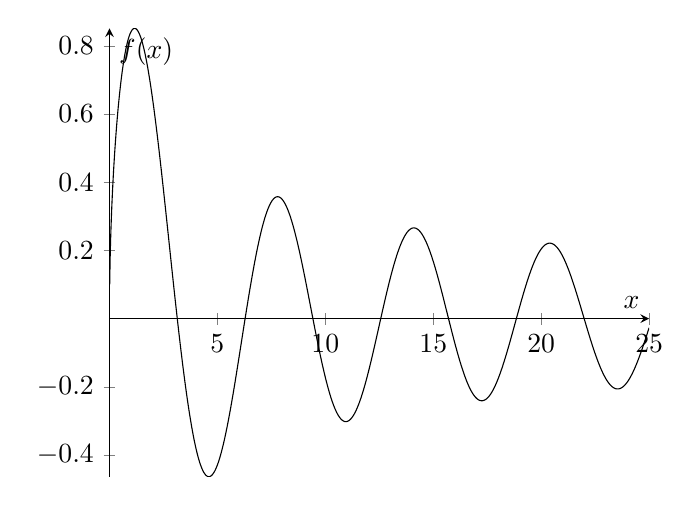
\begin{tikzpicture}
      \begin{axis}[
        xmin = 0, xmax = 25,
        axis x line = middle,
        axis y line = middle,
        xlabel = \(x\),
        ylabel = \(f(x)\)
        ]
        \addplot[
        samples=1000,
        smooth,
        domain=0.01:25] {sin(deg(x))/(sqrt(x))};
      \end{axis}
    \end{tikzpicture}
    \caption{\(f(x) = \frac{\sin(x)}{\sqrt{x}}\)}
  \end{subfigure}
  \caption{\(\Phi_S\)}
\end{figure}


\begin{figure}[!htbp]
  \centering
  \begin{subfigure}{0.45\textwidth}
    \begin{tikzpicture}
      \begin{axis}[
        xmin = -5, xmax = 5,
        axis x line = middle,
        axis y line = middle,
        xlabel= \(x\),
        ylabel= \(\Phi_C(x)\)
        ]
        \addplot[
        samples=100,
        smooth,
        unbounded coords=jump,
        no markers,
        domain = -5:5] gnuplot {FresnelC(x)};
      \end{axis}
    \end{tikzpicture}
    \caption{\(\Phi_C(x)\)}
  \end{subfigure}
  \begin{subfigure}{0.45\textwidth}
    \begin{tikzpicture}
      \begin{axis}[
        xmin = 0, xmax = 25,
        axis x line = middle,
        axis y line = middle,
        xlabel = \(x\),
        ylabel = \(f(x)\)
        ]
        \addplot[
        samples=1000,
        smooth,
        domain=0.38:25] {cos(deg(x))/sqrt(x)};
      \end{axis}
    \end{tikzpicture}
    \caption{\(f(x) = \frac{\cos(x)}{\sqrt{x}}\)}
  \end{subfigure}
  \caption{\(\Phi_C\)}
\end{figure}
